%%=========================================
\section[Diskusjon \& Konklusjon]{Diskusjon \& Konklusjon}
%%=========================================
\subsection{Diskusjon}
{\color{blue}Diskuter resultater. Sammenlign hypoteser og resultater. Diskuter om problemformuleringen er utfordret på en god måte. Sammenligne med teori.}

\subsubsection*{Gestegjenkjennelse gjennom fotodioder}
Dette eksperimentet bestod av følgende:
\begin{itemize}
\item Jeg argumenterte for at en gestesensor i form av enkle fotodioder er et tilstrekkelig medium for enkel brukerinteraksjon.
\item Jeg viste at maskinlæring kan benyttes for å lære et system å forstå enkle gester og viste at dette er et alternativ til å eksplisitt programmere forståelse.
\item Jeg viste at det holder med et titalls treningseksempler fra hver gest for å oppnå gode resultater med lineære modeller, og at det med 50 eksempler oppnås en suksessrate på 96\%.
\end{itemize}

Både logistisk regresjon og støttevektormaskin ga svært lovende resultater, som vist i tabell \ref{table:results}. 96\% er en meget høy suksessrate og viser hvor godt enkle, lineære modeller kan skille på denne typen data. Det ble så interessant å spørre seg om dette resultatet kunne blitt enda høyere. Jeg ønsket ikke å bruke mer tid på å lage flere treningseksempler, så i stedet utførte jeg treningen på nytt med færre treningseksempler, i håp om å kunne se en utviklingstrend. Det samme eksperimentet ble utført med en femtedel og halvparten av dataene for å danne et bilde av sammenhengen mellom forbedring i suksessrate og antall treningseksempler. Figur \ref{figure:resultsgraf} viser resultatene for 100, 250 og 500 treningseksempler. Ettersom biblioteket jeg benyttet for å implementere algoritmene tilbyr en rekke andre algoritmer forsøkte jeg noen andre tilnærminger enn lineære modeller og inkluderte dem også.

I figur \ref{figure:resultsgraf} kan vi se at SVM-ene er i nærheten av 95\% allerede etter 250 treningseksempler og at de kun øker minimalt med 250 ekstra tilfeller. Dette tyder på at det trengs et stort antall ekstra treningseksempler for at algoritmene skal krype betydelig nærmere 100\%. De mer kompliserte algoritmene ExtraTrees og GradientBoost benytter seg av flere algoritmer under panelet og kombinerer disse. Det kan se ut som om spesielt GradientBoost kan fortsette å øke suksessraten betydelig med mer trening, men det er tvilsomt om den noen gang passerer SVM. Til sist nevnes k-nærmeste nabo (kNN), som begynner svakest av de utprøvde algoritmene, men fremdeles har en sterk vekst mellom 250 og 500 tilfeller. Det hadde vært interessant å se utviklingen videre for denne enkle algoritmen.

Dette prosjektet har argumentert for at gester kan være en aktuell interaksjonsform i hjemmet, spesielt som en erstatning til store knappepaneler og desentralisert styringskontroll. Det har også vist at maskinlæring kan benyttes for å gi enkle sensorer en svært god forståelse av gester. Med en suksessrate på over 95\% i klassifiseringen av 10 ulike gester er denne teknikken svært interessant. Og med en suksessrate på over 85\% allerede etter kun 10 treningseksempler på hver gest, kan man forestille seg at brukere selv kan sette av 10 minutter til å trene et helt nytt og utrent system til å forstå sine egne gester. I et produkt kunne det vært aktuelt å tilby online-læring gjennom systemets levetid. Man kan med andre ord la systemet lære etter hvert som brukeren benytter systemet. Dette vil nødvendigvis kreve at brukeren har en mulighet til å gi tilbakemelding på når systemet gjettet riktig gest og når det gjettet feil. Jeg har vist at en enkel sensor, gjennom maskinlæring, kan benyttes praktisk som en multifunksjonell bryter med flere tilstander enn hva man kan programmere for hånd.


\subsubsection*{Multimodal interaksjon gjennom tale og gester}
Eksperimentet hadde følgende utfall:
\begin{itemize}
\item Jeg argumenterte for at tale og gester fungerer best i kommunikasjonsprogramvare.
\item Jeg argumenterte for at kombinasjonen av enkle gester og talekommandoer er en effektiv måte å interagere med det smarte hjemmet på.
\item Jeg viste at talegjenkjenning over en begrenset mengde ord dekker funksjonaliteten vi ønsker å tilby gjennom tale, og at det finnes åpne og tilgjengelige løsninger for å løse dette problemet.
\item Jeg implementerte et system som håndterer multimodal inputdata fra gestesensor og mikrofon. Denne ble benyttet for å simulerer bruken i et smart hjem ved å vise en dynamisk grafisk representasjon av inputdataene.
\end{itemize}

Vi kan si at hypotesen er godt utfordret dersom den multimodale interaksjonen kan vises å være tilstrekkelig til å styre hjemmet, at den er naturlig og at den er effektiv. Disse er vanskelige å måle empirisk. Eksperimentet har argumentert for at den begrensede talegjenkjenningen ikke bare er tilstrekkelig, men er en bedre tilnærming enn kontinuerlig tale, med dagens begrensninger i teknologi. Med definisjonene for naturlig og effektiv jeg ga i kapitell 1 trengs det eksperimenter med brukere for å besvare hypotesen. For å avgjøre om interaksjonen er instinktiv, forståelig, enkel i bruk, praktisk og hensiktsmessig må et bredt utvalg brukere observeres mens de tar i bruk systemet. Jeg definerte også ordene slik at de naturlig interaksjon må gi rimelige resultater og effektiv interaksjon må gi resultater raskt. I kontekst av det smarte hjemmet kan disse kravene være vanskelig å oppfylle. Dersom du sier til hjemmet at lyset skal skrus av i rommet brukeren befinner seg i kan resultat evalueres umiddelbart. Men dersom brukeren bruker systemet for å låse ytterdøra, senke temperaturen eller slå av lyset i et annet rom er det en utfordring å for dette systemet å gi feedback raskt, og å gi feedback som forteller brukeren om resultatet var rimelig.

\subsubsection*{Kombinasjoner}
Eksperimentet hadde følgende utfall:
\begin{itemize}
\item Jeg argumenterte for at et stort vokabular av abstrakte gester i praksis er et tegnspråk og at retningslinjer som gjelder for taledrevne systemer også gjelder for slike gestedrevne systemer.
\item Jeg viste at de 10 gestene fra eksperiment 1 over fire sensorer, danner langt bedre data og at maskinlæring er enda mer effektivt.
\item Jeg viste at systemet kan trenes til å skille mellom 42 ulike gester med 94\% suksessrate, etter å kun ha sett 10 treningseksempler av hver gest.
\item Jeg argumenterte for at sensorenes andre egenskaper, som nærhetsdeteksjon og mål av lysnivåer, kan brukes i forbindelse med smarte hjem, blant annet for å dimme lys og regulere lydvolum.
\end{itemize}

Diskusjon og sammenligning hypotese og resultat, problemstilling utfordret godt?
Resultatet fra maskinlæringen stemmer godt overens med hypotesen. Om de 42 gestene er naturlige er ikke bestemt. Her trengs det data fra brukere for å gi et betydelig svar. Det er klart de ulike gestene og hva de eventuelt styrer kan læres. Men om de ulike måtene å sveipe hånda delvis over sensorer eller med forskjellige hastigheter er intuitiv, er svært diskutabelt.

Å utnytte nærhetssensoren for å lage funksjonalitet for å dimme lys, heve og senke persienner og regulere lydvolum vil jeg si er av verdi.

\subsubsection*{Kontekstdrevet brukergrensesnitt}
Eksperimentet hadde følgende utfall:
\begin{itemize}
\item Jeg argumenterte for at et grafisk brukergrensesnitt for smarte hjem er informasjonsprogramvare. Brukerene er hovedsaklig interessert i å lære om hjemmet og informasjonen bør derfor presenteres på en optimal måte.
\item Jeg implementerte et prototypesystem som viser hjemmets tilstand og dynamisk tilpasser seg ny informasjon. Grensesnittets utseende forandret seg basert på regler og prioriteringer.
\end{itemize}

{\color{blue}Diskusjon og sammenligning hypotese og resultat, problemstilling utfordret godt?

Sammenligne med definisjonen av intelligente brukergrensesnitt fra introduksjonen og diskuter om jeg har brukt teknikker fra IUI for å lage et godt grensesnitt.}

\subsection{Videre arbeid}
{\color{blue}Ting fra teori jeg kunne gjort?}

\subsubsection*{Gestegjenkjennelse gjennom fotodioder}
Tre viktige valg ble tatt i dette eksperimentet: hvilke klassifiseringslagoritmer som ble utforsket, antall treningseksempler, og antallet datapunkter valgt i datavektorene systemet ble trent med. Alle disse dimensjonene ville vært interessante å utforske med andre valg. Vil andre algoritmer fungerere bedre dersom antallet treningseksempler øker? Teknikker som dyp læring med nevrale nett kan tilnærme mer avanserte funksjoner med tilstrekkelig trening. Og kunne resultatene vært bedre med større datavektorer? Med gestene som skaper mye datapunkter blir datavektorene gjennomsnittsresultater og vi mister en del presisjon i dataene. Større datavektorer vil kreve flere ressurser fra systemet.

Til sist vil jeg også nevne online læring. Man kan utforske et system som lærer etter hvert som brukeren bruker systemet. For å få feedback er brukeren da nødt til å kunne gi beskjed om systemet gjettet riktig gest eller ikke. Kan dette utføres med talegjenkjenning og syntesert tale? Et annet alternativ er en liten touchskjerm der brukeren kan svare på om gesten ble gjettet riktig.

\subsubsection*{Multimodal interaksjon gjennom tale og gester}
Det umiddelbare videre arbeid for den begrensede talegjenkjenningen virker ganske klart: å implementere "rejecting out of grammar utterances". Slik systemet står nå vil enhver lyd gjenkjennes som et av ordene eller uttrykkene i vokabularet. Når usikkerheten om en lyd er stor bør en null-verdi gjettes. Dermed unngår man at kremt, host, bakgrunnsstøy og pauselyder blir feilaktig gjenkjent som talekommandoer. Dette er ikke implementert i Pocketsphinx ennå.

Et spennende prosjekt ville vært å kombinere begrenset tale for å gi hjemmet kommandoer og kontinuerlig, naturlig tale for å spørre orakelspørsmål, som "hva er værmeldingen for neste fredag?" eller "finn en oppskrift på tacokrydder.". En idé er å la ulike aktiveringsgester aktiver den passende talegjenkjenningen. Ved å utføre den riktige gesten vil systemet, i stedet for den lokale talegjenkjenningen, åpne opp en kobling til en tjeneste, som Google, og lytte etter input.
enkle kommandoer for å styre hjemmet, naturlig tale for å spørre orakel-spørsmål.
 
Andre alternativer for å løse problemet med å håndtere input fra flere kanaler.

Brukertesting. Vil brukere finne det naturlig å prate for å skru av og på apparatene i hjemmet? Er det fordelaktig å ha et sentralt, eller et fåtall sentrale steder å utøve styring fra?

\subsubsection*{Kombinasjoner}
Når vi nå har etablert at disse sensorene kan oppnå en forståelse for gester ved hjelp av maskinlæring, dukker det opp andre bruksområder. Spesielt situasjoner der det er fordelaktig å unngå fysisk kontakt er interessante. Et eksempel er toaletter og vasker, der en enkel gest kan skylle ned eller starte vannet, og andre gester kan justere vanntemperaturen. Et annet sted der hygiene er svært viktig er på sykehus. Jeg kan forestille meg at det ville være aktuelt for helsepersonell å styre ulik funksjonalitet på et sykehus, uten å komme i kontakt med knapper, skjermer og dører. Her er det store muligheter for utforskning.

Dersom man benytter systemet slik at det må både tale og gester til for å aktivere funksjonalitet, har man i praksis en 2-veis autentisering. Dette kan dermed brukes som en sikkerhetsmekanisme. Kanskje en lås åpnes, eller tilgang til å styre funksjonalitet i hjemmet gis, ved å si en passord-frase av vilkårlig lengde sammen med en eller flere korrekte gester. Dette vil være en svært trygg autentisering, og den er samtidig effektiv å utføre og krever ikke tilgang til et tastatur.

Et aktuelt applikasjonsområde å utforske for sensorene er i forbindelse med tablets. Hva kunne man fått til dersom en tablet hadde slike sensorer plassert for eksempel i hjørnene, på kantene eller på baksiden? Gester kunne brukes for å utføre vanlige funksjoner som å scrolle og å navigere mellom app'er eller nettleserfaner. Men kanskje helt nye interaksjonsformer nå kunne blitt utforsket. Kunne man utnyttet abstrakte gester i luftrommet rundt tableten for å skape god interaksjon?

Både tale og gester fungerer best for å gi kommandoer. Mange manipulasjonsprogrammer i dag har store menyer med verktøy og instillinger man skal velge i. Kunne man benyttet mer av skjermarealet til det primære utviklingsområdet ved å tilby valg av verktøy og instillinger gjennom tale og gester?

\textbf{Lys og fargenivå}\newline
\begin{figure}[h]
\centering
\begin{subfigure}{0.23\textwidth}
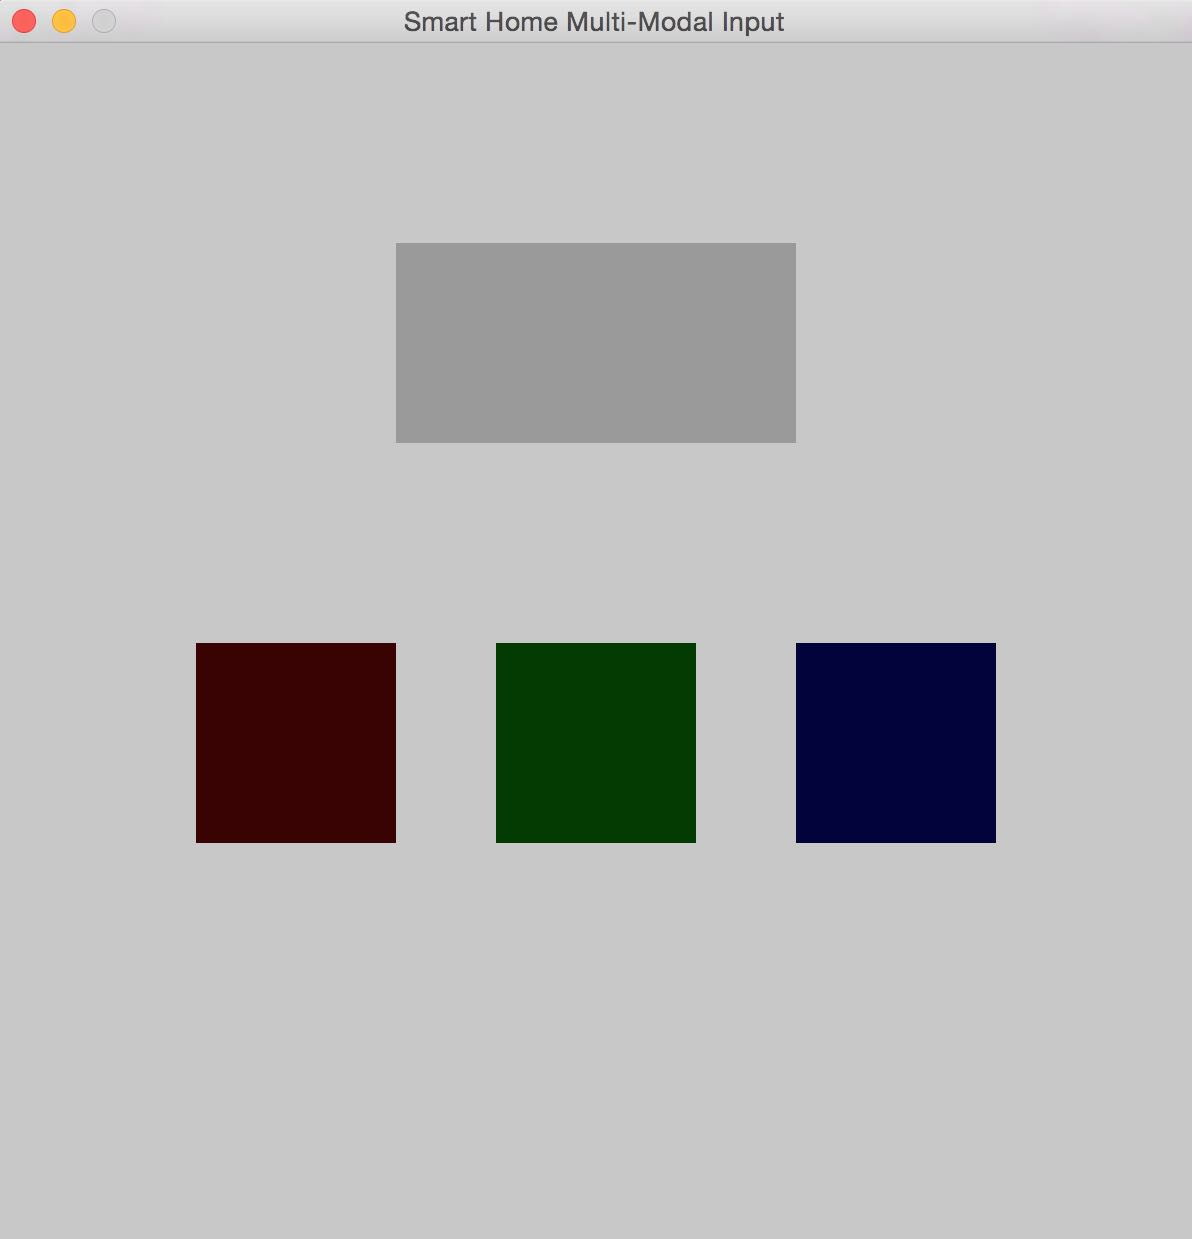
\includegraphics[width=3cm, height=3cm]{fig/color-1}
\caption{}
\label{fig:color-1}
\end{subfigure}
\begin{subfigure}{0.23\textwidth}
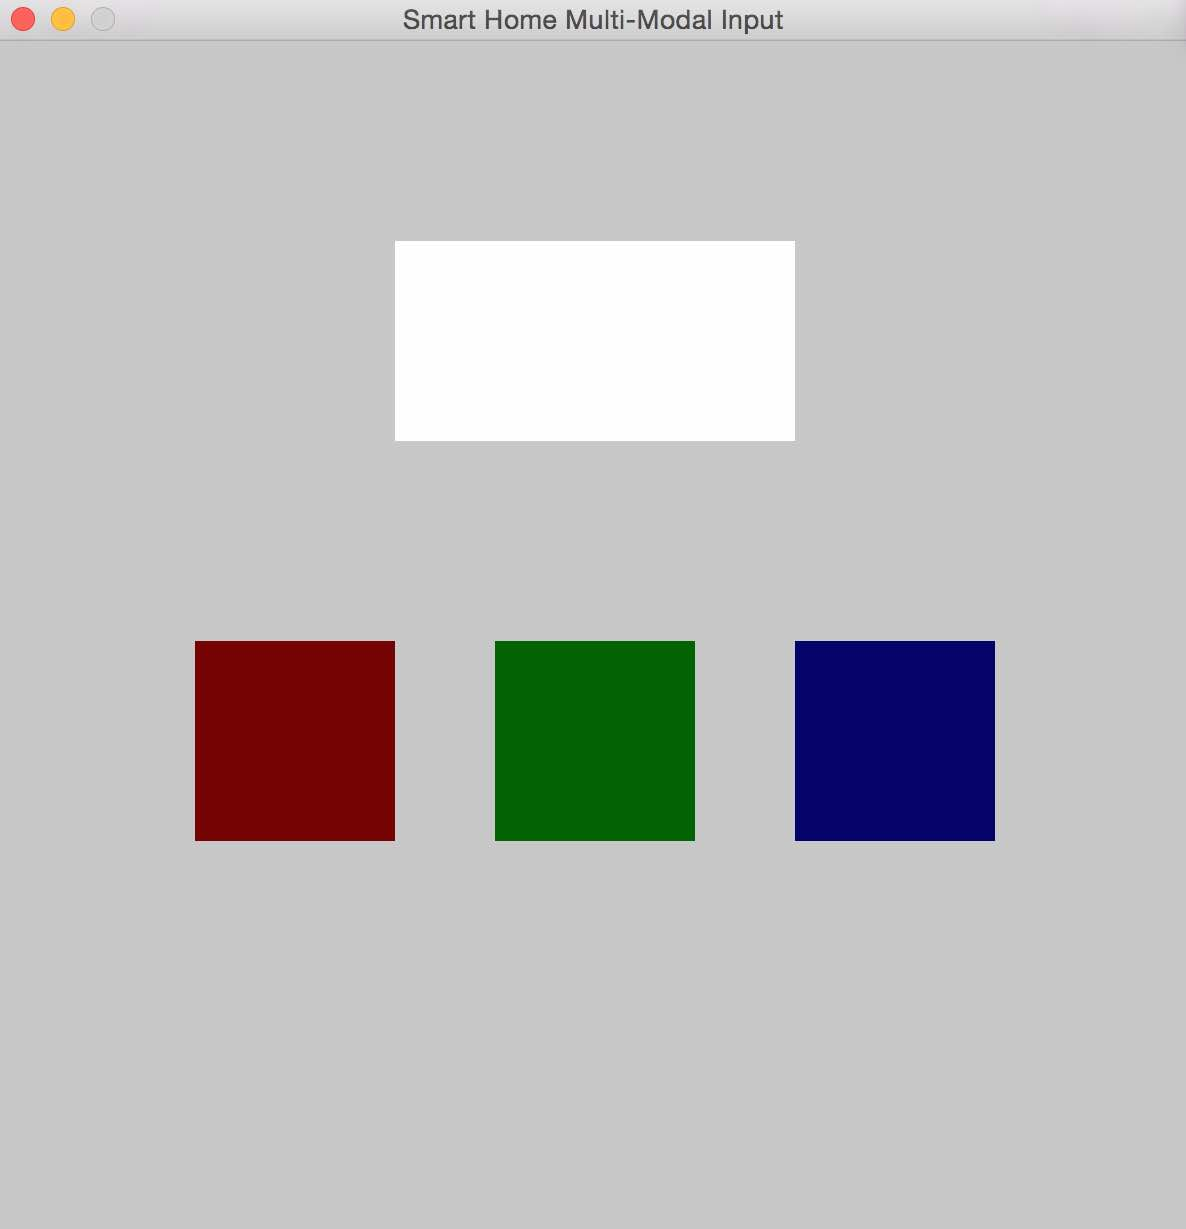
\includegraphics[width=3cm, height=3cm]{fig/color-2}
\caption{}
\label{fig:color-2}
\end{subfigure}
\begin{subfigure}{0.23\textwidth}
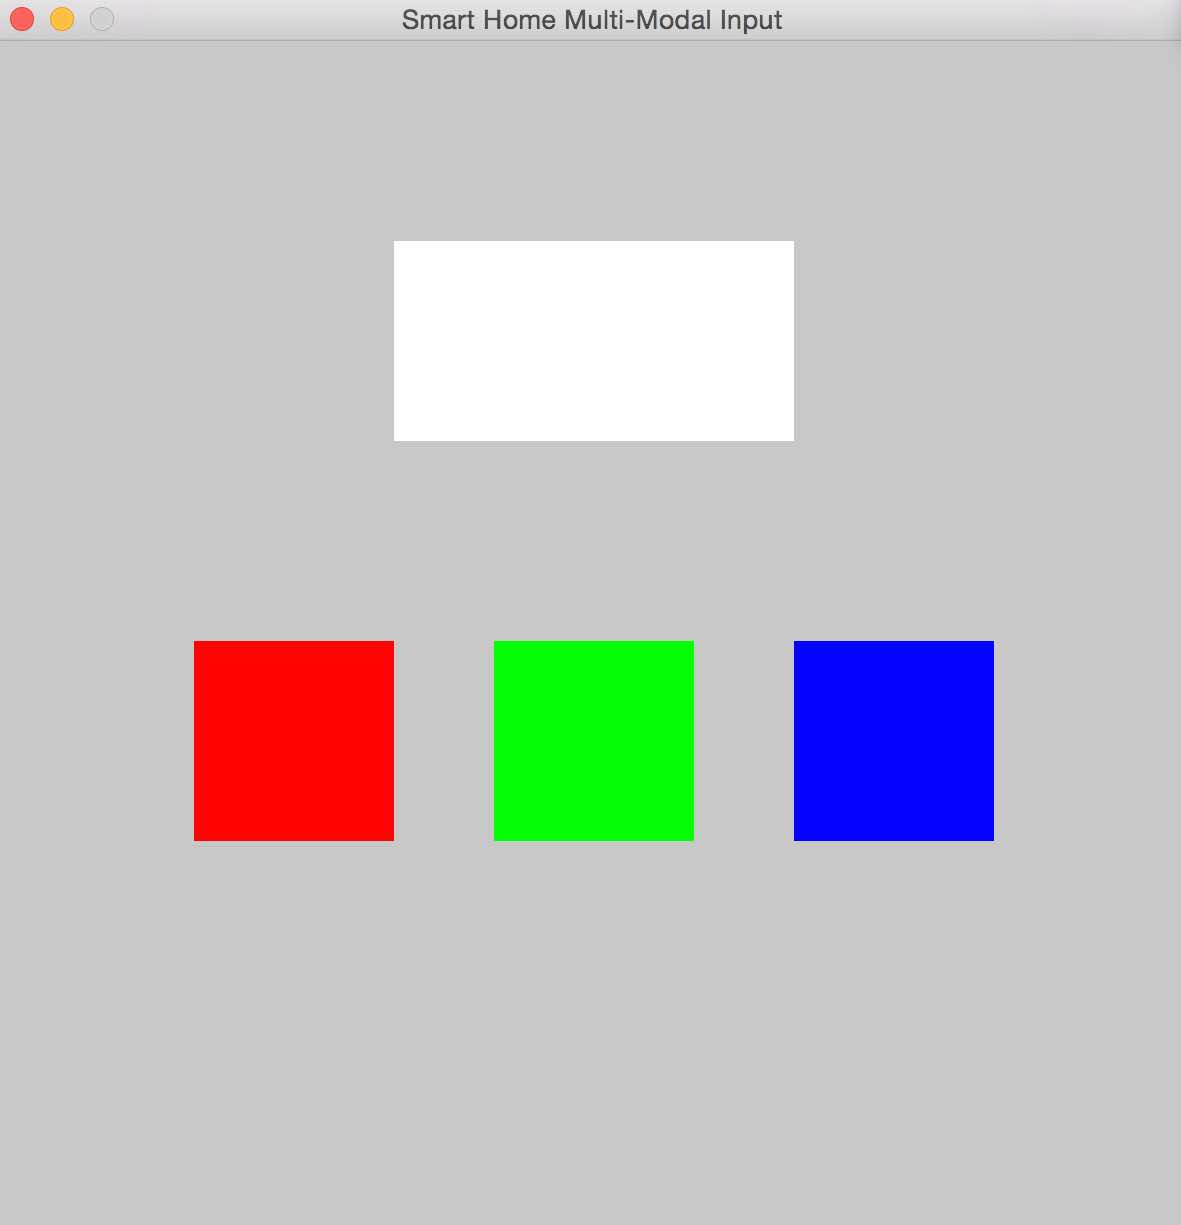
\includegraphics[width=3cm, height=3cm]{fig/color-3}
\caption{}
\label{fig:color-3}
\end{subfigure}
\caption{Lys og fargenivå.}
\label{fig:color}
\end{figure}

\subsubsection*{Kontekstdrevet brukergrensesnitt}
For å gi brukergrensesnittet en grad av intelligens ble det implementert et utvalg regler. Disse definerte hvilken informasjon som var av prioritet og som skulle presenteres for brukeren. En videre utvikling kunne være å la brukere legge inn egne regler, og selv definere hva som er viktigst. Videre kunne teknikker fra maskinlæring også her benyttes for å la programmet selv lære hva brukeren foretrekker. 

Å knytte brukergrensesnittet til reell sensordata ville vært et viktig steg videre. Man kunne så utforsket hvordan brukere benyttet systemet til å få svar på det de leter etter. Brukertesting med både tradisjonelle interaksjonsdrevne grensesnitt, samt et kontekstdrevet, ville kunne hentet empiriske data på om denne tilnærmingen er bedre.

\subsection{Konklusjon}
{\color{red}Sammenlign arbeid med mål og teori!}\newline
{\color{blue}Hovedmålene for denne oppgaven er å:
\begin{itemize}
\item Benytte maskinlæring for å utvide egenskapene og bruksområdene til enkle sensorer.
\item Eksperimentere med håndtering av samtidig input fra både gester og begrenset tale.
\item Utfordre nåværende grafiske brukergrensesnitt for smarte hjem, ved å lage programvare drevet av kontekst framfor interaksjon.
\end{itemize}}

Denne oppgaven har tatt for seg et utvalg tilnærminger til brukergrensesnitt i smarte hjem. Jeg valgte å ta utgangspunkt i en tredeling av typer programvare: programvare for informasjons, manipulasjons og kommunikasjons. Denne inndelingen gjorde at jeg kunne identifisere og kategorisere ulike aktuelle intelligente brukergrensesnitt. Etter å ha kategorisert en interaksjonsmetode som en bestemt type programvare var det enklere å argumentere for hvordan interaksjonsmetoden burde benyttes.

Målene for oppgaven var i utgangspunktet noe høytsvevende og vanskelig å måle. Til gjengjeld var de spesifikke hypotesene mer konkrete og målbare. I den foregående diskusjonen argumenterte jeg for hvordan hypotesene ble utfordret på en god måte. Det første målet var å benytte maskinlæring til å gi enkle sensorer utvidet funksjonalitet. Dette målet ble fullført gjennom eksperimentene 1 og 3 der dataene fra relativt enkle gestesensorer ble tilpasset og brukt i lineære klassifiseringsalgoritmer. Resultatene var svært lovende og viser hvordan maskinlæring kan gi større funksjonalitet enn det vi kan eksplisitt programmere. Det andre målet var å eksperimentere med multimodal input. Jeg ønsket å finne en enkel, men tilstrekkelig måte å håndtere input fra gester og tale samtidig. Å benytte køer og tråder løser problemet med å håndtere asynkron input. Men det ser ikke nærmere på elementer som ble omtalt i teorien, som å forbedre forståelse eller å velge den beste inputen fra flere kanaler. På dette viset er dette målet ikke tilstrekkelig utforsket i oppgaven. Jeg endte i stedet opp med å fokusere på problemene med kontinuerlig tale og hvordan begrenset tale kan benyttes.

Fra bakgrunnsteorien lærte vi om tilnærming gjennom agenter for å håndtere grensesnittet. Min løsning er også her enklere, men i min mening ikke svakere. Å introdusere agenter kan gjøre systemet mer komplekst. Dersom hver agent er godt adskilt og all kommunikasjon er gjennom meldinger kan kompleksiteten holdes lav. Men agentene i \citet{ishizaki96} virker sammenkoblede i den forsand at de selv må forholde seg til hverandre. En slik løsning er unektelig mer dynamisk og systemet kan selv komme opp med ny måter å presentere data på. Jeg er usikker på om dette vil gi tilstrekkelig gode resultater i et brukergrensesnitt for smarte hjem. Dersom målet er å vise dataene på en best mulig måte har jeg større tro på en kompetent grafisk designer, enn et sett av agenter som skal samarbeide om å vise informasjonen på en optimal måte. 


